\documentclass[a4paper,12pt]{article}

\usepackage[
    left=2cm,
    right=2cm,
    top=3cm,
    bottom=3cm
]{geometry}

\usepackage[utf8]{inputenc}
\usepackage[czech]{babel}
\usepackage[T1]{fontenc}
\usepackage{graphicx}
\usepackage{array}
\usepackage{booktabs}
\usepackage{tabularx}
\usepackage{makecell}
\usepackage{float}
\usepackage{newunicodechar}
\usepackage{url}
\usepackage{siunitx}
\usepackage{listings}
\usepackage{xcolor}
\usepackage{diagbox}
\usepackage{hyperref}
\usepackage{tikz}
\usepackage{pgfplots}
\pgfplotsset{compat=1.18}

\usepackage{fancyhdr}
\pagestyle{fancy}

\fancyhf{}
\fancyhead[L]{Studium fotoefektu a stanovení Planckovy konstanty}
\fancyhead[R]{Pavel Pernička}
\fancyfoot[C]{\thepage}

\fancypagestyle{firstpage}{
    \fancyhf{}
    \renewcommand{\headrulewidth}{0pt}
    \renewcommand{\footrulewidth}{0pt}
    \fancyfoot[C]{\thepage}
}

\definecolor{myblue}{RGB}{111,0,248}
\newcommand{\colorcircle}[1]{%
  \tikz[baseline=-0.6ex]\draw[fill=#1,draw=none] (0,0) circle (1.5ex);%
}
\newcommand{\unitC}{\,^\circ\mathrm{C}}
\newcommand{\unitV}{\,\mathrm{V}}
\newcommand{\unitA}{\,\mathrm{A}}
\newcommand{\units}{\,\mathrm{s}}
\newcommand{\unitmin}{\,\mathrm{min}}

\newcommand{\centered}[1]{\begin{tabular}{l} #1 \end{tabular}}

\addto\captionsczech{\renewcommand{\refname}{Seznam použité literatury}}
\addto\captionsczech{\renewcommand{\figurename}{\textbf{Obrázek}}}
\addto\captionsczech{\renewcommand{\tablename}{\textbf{Tabulka}}}
\renewcommand{\lstlistingname}{\textbf{Kód}}

\lstset{
    language=Python,
    basicstyle=\ttfamily\footnotesize,
    keywordstyle=\color{blue},
    commentstyle=\color{gray},
    stringstyle=\color{red},
    numbers=left,
    numberstyle=\tiny\color{gray},
    stepnumber=1,
    breaklines=true,
    frame=single
}

\begin{document}
\thispagestyle{firstpage}

\vspace*{\fill}
\begin{center}
\renewcommand{\arraystretch}{1.75}

\begin{tabularx}{\textwidth}{|X|X|X|}
    \hline
    \multicolumn{1}{|c|}{\rule{0pt}{2.25cm} 
\includegraphics[height=2cm]{img/ctu_logo.png}}
    & \multicolumn{2}{c|}{\makecell{\textbf{KATEDRA FYZIKY}}} \\
    \hline
    \multicolumn{3}{|c|}{\Large \textbf{\centered{LABORATORNÍ CVIČENÍ Z FYZIKY}}} \\
    \hline
    \multicolumn{2}{|X}{\small{Jméno} \newline \textbf{Pavel Pernička}}
    & \multicolumn{1}{|X|}{\small{Datum měření} \newline \textbf{25.11.2025}} \\
    \hline
    {\small{Semestr} \newline \textbf{Zimní 2025}}
    & {\small{Ročník} \newline \textbf{2.}}
    & {\small{Datum odevzdání} \newline \textbf{23.12.2025}} \\
    \hline
    {\small{Stud. skupina} \newline \textbf{6}}
    & {\small{Lab. skupina} \newline \textbf{1061}}
    & {\small{Klasifikace} \newline} \\
    \hline
    \multicolumn{3}{|c|}{\rule{0pt}{1cm}} \\
    \hline
    \multicolumn{1}{|X|}{\small{Číslo úlohy \newline \textbf{8}}}
    & \multicolumn{2}{|p{9cm}|}{\small{Název úlohy \newline \textbf{Studium fotoefektu a stanovení Planckovy konstanty -- hodnoty}}} \\
    \hline
\end{tabularx}

\end{center}
\vspace*{\fill}

\newpage
\section{Úkol měření}
\begin{itemize}
  \item Na základě měření vnějšího fotoelektrického jevu stanovte velikost Planckovy konstanty~$h$.
  \item Určete mezní kmitočet a výstupní práci materiálu fotokatody použité fotonky. Porovnejte tuto hodnotu s výstupními pracemi jiných materiálů a odhadněte, z jakého materiálu je tato fotokatoda vyrobena.
  \item Určete nejistotu měření pro všechny veličiny určené v bodech 1 a~2.
  \item Vypracujte graf závislosti maximální kinetické energie elektronů na frekvenci záření
  \[
    W_k = f(\nu).
  \]
  \item Změřte závislost fotoelektrického proudu na velikosti brzdného potenciálu pro tři vlnové délky.
  \item Do jednoho grafu vyneste pro všechny tři vlnové délky změřené závislosti fotoelektrického proudu na velikosti brzdného potenciálu.
  \item Porovnejte hodnotu změřené Planckovy konstanty s tabulkovou hodnotou a rozdíl zhodnoťte.
  \item Měření a zpracování dat v bodech 1--7 proveďte zvlášť pro obě instalované měřicí aparatury, závislost $W_k = f(\nu)$ vyneste do jednoho (společného) grafu. Body 5--6 provádějte pouze pro soupravu se spektrálním fotometrem Spekol.
\end{itemize}

\section{Seznam použitých přístrojů}
\begin{itemize}
    \item Spektrální fotometr Spekol
        \begin{itemize}
            \item Velikost nejmenšího dílku ampérmetru : $1\ \unit{\mu A}$,
            \item Velikost nejmenšího dílku vlnové délky : $1\ \unit{nm}$.
        \end{itemize}
    \item Souprava s výbojkou a monochromatickými filtry.
    \item 2x digitální multimetr.
\end{itemize}

\newpage
\section{Naměřené hodnoty}

\subsection{Spektrální fotometr Spekol}

\begin{table}[H]
\centering
\renewcommand{\arraystretch}{1.5}
\begin{tabular}{|c|c|c|c|c|c|}
\hline
$I\ [\mu\mathrm{A}]$ &
$\lambda=375\,\mathrm{nm}$ &
$\lambda=400\,\mathrm{nm}$ &
$\lambda=425\,\mathrm{nm}$ &
$\lambda=450\,\mathrm{nm}$ &
$\lambda=475\,\mathrm{nm}$ \\
\hline
100 & -0.0023 & 0.0017 & -0.0044 & -0.0007 & 0.0010 \\
90  & 0.0615  & 0.0550 & 0.0481  & 0.0475  & 0.0446 \\
80  & 0.1252  & 0.1213 & 0.1031  & 0.0961  & 0.0843 \\
70  & 0.1929  & 0.1808 & 0.1580  & 0.1489  & 0.1299 \\
60  & 0.2677  & 0.2490 & 0.2164  & 0.1995  & 0.1758 \\
50  & 0.3467  & 0.3126 & 0.2797  & 0.2567  & 0.2241 \\
40  & 0.4405  & 0.3952 & 0.3470  & 0.3161  & 0.2737 \\
30  & 0.5582  & 0.4755 & 0.4214  & 0.3784  & 0.3335 \\
20  & 0.6772  & 0.5985 & 0.5223  & 0.4602  & 0.4031 \\
10  & 0.8547  & 0.7393 & 0.6500  & 0.5627  & 0.4982 \\
0   & 1.2550  & 1.0802 & 0.9352  & 0.8322  & 0.7163 \\
\hline
\end{tabular}
\caption{Naměřená brzdná napětí $U_p$ pro různý fotoelektrický proud na fotometru Spekol}
\end{table}

\subsection{Souprava s monochromatickými filtry}

\begin{table}[H]
\centering
\renewcommand{\arraystretch}{1.5}
\begin{tabular}{|c|c|c|c|c|c|}
\hline
 & $\lambda = 0\,\mathrm{nm}$ & $\lambda = 578\,\mathrm{nm}$ & $\lambda = 546\,\mathrm{nm}$ & $\lambda = 436\,\mathrm{nm}$ & $\lambda = 408\,\mathrm{nm}$ \\
\hline
$U_p\,[\mathrm{V}]$     & 0.005 & 0.272 & 0.396 & 0.849 & 1.052 \\
$\text{offset}\,[\mathrm{V}]$ & 0.010 & 0.004 & 0.001 & 0.008 & -0.003 \\
\hline
\end{tabular}
\caption{Naměřená brzdná napětí a jednotlivé offsety pro soupravu s filtry}
\end{table}

\newpage
\section{Zpracování naměřených hodnot}

\subsection{Kmitočet dopadajícího záření a kinetická energie elektronů}

Maximální kinetická energie elektronů je dána vztahem
\[
W_k = e U_p,
\]
kde $e$ je elementární náboj a $U_p$ brzdné napětí. Pokud energii vyjadřujeme
v~elektronvoltech, platí jednoduše
\[
W_k\,[\mathrm{eV}] = U_p\,[\mathrm{V}].
\]

Frekvence dopadajícího světla je
\[
\nu = \frac{c}{\lambda},
\]
kde $c$ je rychlost světla a $\lambda$ je vlnová délka. U soustavy s filtry jsou brzdná napětí nejdříve posunuta o změřený offset a až pak se z nich počítá energie $W_k$.
\[
U_{\text{kor}} = U_p - U_{\text{offset}},
\]

\begin{table}[H]
\centering
\renewcommand{\arraystretch}{1.5}
\begin{tabular}{|c|c|c|c|}
\hline
$\lambda\,[\mathrm{nm}]$ & $U_p\,[\mathrm{V}]$ &
$\nu\,[\mathrm{PHz}]$ & $W_k\,[\mathrm{eV}]$ \\
\hline
375 & 1.2550 & 0.799 & 1.2550 \\
400 & 1.0802 & 0.750 & 1.0802 \\
425 & 0.9352 & 0.705 & 0.9352 \\
450 & 0.8322 & 0.666 & 0.8322 \\
475 & 0.7163 & 0.631 & 0.7163 \\
\hline
\end{tabular}
\caption{Dopočítané frekvence a kinetické energie -- Spekol}
\end{table}

\begin{table}[H]
\centering
\renewcommand{\arraystretch}{1.5}
\begin{tabular}{|c|c|c|c|c|c|}
\hline
$\lambda\,[\mathrm{nm}]$ &
$U_p\,[\mathrm{V}]$ &
$U_{\text{offset}}\,[\mathrm{V}]$ &
$U_{\text{kor}}\,[\mathrm{V}]$ &
$\nu\,[\mathrm{PHz}]$ &
$W_k\,[\mathrm{eV}]$ \\
\hline
578 & 0.272 & 0.004 & 0.268 & 0.519 & 0.268 \\
546 & 0.396 & 0.001 & 0.395 & 0.549 & 0.395 \\
436 & 0.849 & 0.008 & 0.841 & 0.688 & 0.841 \\
408 & 1.052 & -0.003 & 1.055 & 0.735 & 1.055 \\
\hline
\end{tabular}
\caption{Brzdná napětí, frekvence a energie -- souprava s filtry}
\end{table}

\section{Určení Planckovy konstanty a výstupní práce}

Z Einsteinova vztahu pro fotoefekt
\[
W_k = h \nu - A = e U_p
\]
vyplývá, že závislost $W_k(\nu)$ by měla být lineární. Toho využijeme a metodou nejmenších čtverců proložíme naměřené body polynomem prvního řádu a pomocí skriptu dostaneme směrnice a~offset. Pro Spekol jsou hodnoty:

$$
W_k = (3.16\,\nu - 1.28)\ \mathrm{eV},
$$

Odtud:

$$
h_s = 1.602\times 10^{-34}\cdot 3.16
      = 5.07\times 10^{-34}\ \mathrm{J\,s},
$$
$$
A_s = 1.28\ \mathrm{eV}.
$$

A pro soupravu s filtry jsou hodnoty:
$$
W_k = (3.52\,\nu - 1.55)\ \mathrm{eV},
$$

Odtud:

$$
h_f = 1.602\times 10^{-34}\cdot 3.52
      \approx 5.64\times 10^{-34}\ \mathrm{J\,s},
$$
$$
A_f = 1.55\ \mathrm{eV}.
$$

\section{Závislosti a grafy}

\subsection{Závislost maximální kinetické energie na frekvenci záření}

\begin{figure}[H]
\centering
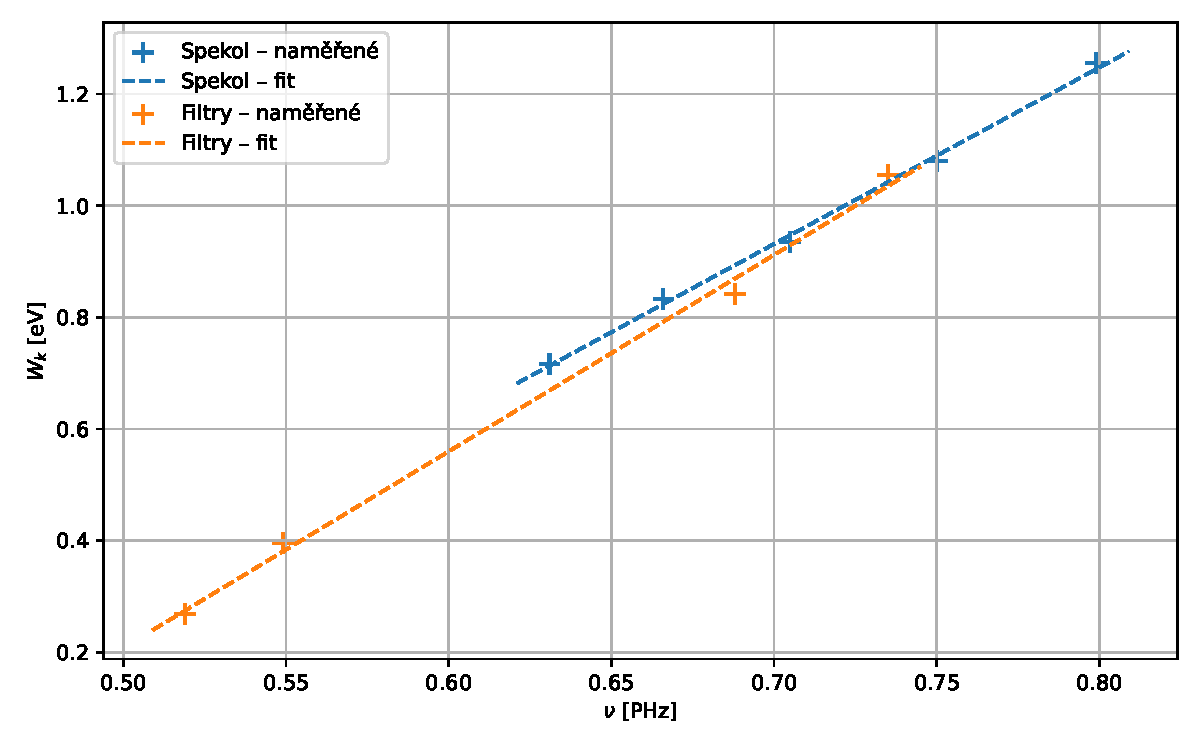
\includegraphics[width=\textwidth]{img/wk_vs_nu.pdf}
\caption{Závislost maximální kinetické energie elektronů na frekvenci záření}
\end{figure}

\subsection{Závislost fotoelektrického proudu na brzdném napětí}

\begin{figure}[H]
\centering
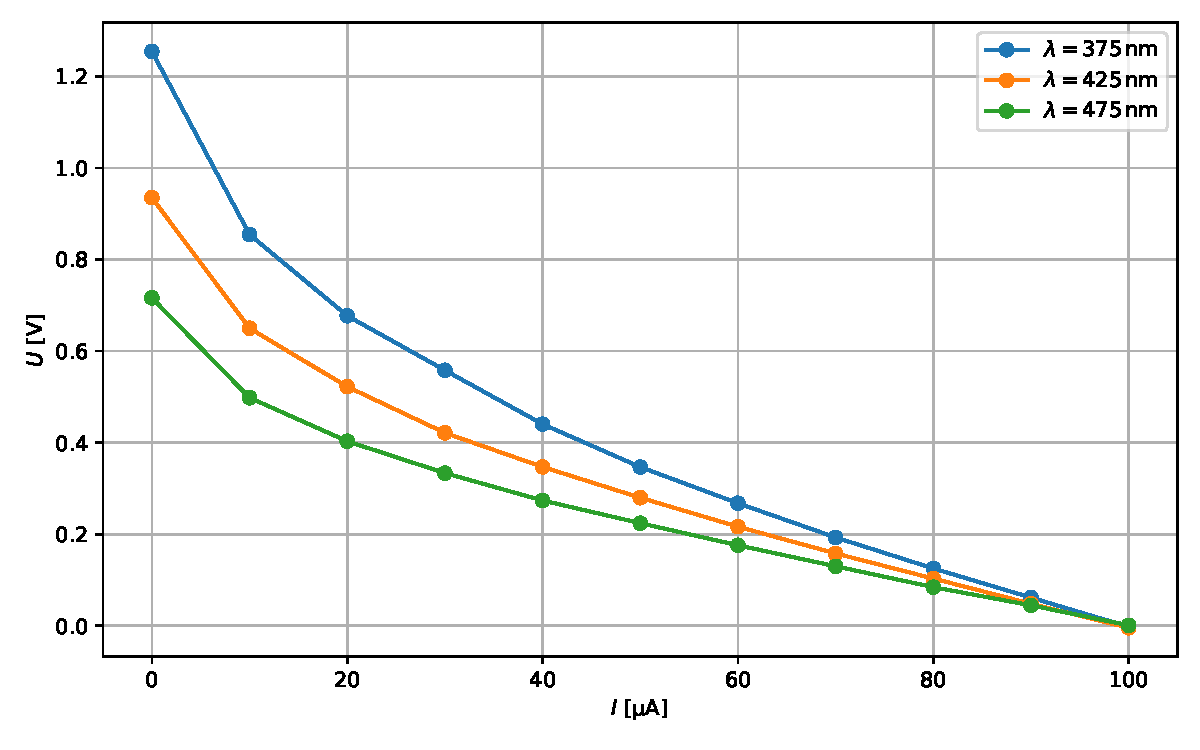
\includegraphics[width=\textwidth]{img/U_vs_I.pdf}
\caption{Závislost fotoelektrického proudu na brzdném napětí pro vybrané vlnové délky}
\end{figure}

\section{Závěr}

Na základě měření vnějšího fotoelektrického jevu byly pro dvě různé
měřicí soustavy určeny hodnoty Planckovy konstanty
\[
h_s \approx 5.1\times 10^{-34}\ \mathrm{J\,s} \quad\text{(Spekol)},\qquad
h_f \approx 5.6\times 10^{-34}\ \mathrm{J\,s} \quad\text{(filtry)}.
\]
Obě hodnoty jsou nižší než tabulková hodnota
\[
h_\mathrm{real} = 6.626\times 10^{-34}\ \mathrm{J\,s},
\]

Výstupní práce fotokatody byla odhadnuta jako
\[
A_s \approx 1.3\ \mathrm{eV} \quad\text{(Spekol)},\qquad
A_f \approx 1.6\ \mathrm{eV} \quad\text{(filtry)},
\]
což odpovídá materiálům s nízkou výstupní prací, kde obecně spadají alkalické kovy.

\newpage
\section{Přílohy}
\begin{itemize}
    \item Foto záznamového papíru s hodnotami
\end{itemize}

\begin{thebibliography}{}

    \bibitem{zadani}
    Milan Červenka. \textit{Studium fotoefektu a stanovení Planckovy konstanty}. Laboratorní úloha, 2019. Dostupné online: \url{https://planck.fel.cvut.cz/praktikum/downloads/navody/planck.pdf}.

    \bibitem{skripta}
    Michal Bednařík. \textit{Studijní texty k předmětu Fyzika 2}.
    
    \bibitem{zpracdat}
    Milan Červenka. \textit{Zpracování fyzikálních měření}. Studijní text pro fyzikální praktikum, 2020. Dostupné online: \url{https://planck.fel.cvut.cz/praktikum/downloads/navody/zpracdat.pdf}.

\end{thebibliography}

\end{document}
